% Master Thesis LaTeX Template
% Collaboration: VU Amsterdam, University of Amsterdam (UvA), DTU Denmark

\documentclass[12pt,twocolumn]{article}

\usepackage[numbers,sort&compress]{natbib}
% Encoding and Language
\usepackage[utf8]{inputenc}
\usepackage[T1]{fontenc}
\usepackage[english]{babel}
\usepackage{booktabs}
\usepackage{amsmath}
\usepackage{tikz}
\usetikzlibrary{positioning}


% Page Layout and Spacing
\usepackage{geometry}
\geometry{a4paper, margin=1in}
\usepackage{setspace}
\onehalfspacing

% Graphics and Logos
\usepackage{graphicx}
\usepackage{float}

% Hyperlinks
\usepackage{hyperref}
\hypersetup{
  colorlinks=true,
  linkcolor=blue,
  citecolor=blue,
  urlcolor=blue
}

%----------------------------------------------------------------------------------------
% DOCUMENT INFORMATION
%----------------------------------------------------------------------------------------
\title{\bfseries Title of Your Master Thesis}
\author{Your Name}
\date{\today}

%----------------------------------------------------------------------------------------
% BEGIN DOCUMENT
%----------------------------------------------------------------------------------------
\begin{document}

%----------------------------------------------------------------------------------------
% TITLE PAGE
%----------------------------------------------------------------------------------------
\begin{titlepage}
  \centering
  % Logos: place your logo files in a 'logos/' folder
\begin{figure}[H]
  \centering
  % first logo
  \begin{minipage}[c]{0.30\linewidth}
    
\includegraphics[height=1.4cm]{figures/logo/vu-griffioen.pdf}
  \end{minipage}
  \hfill
  % second logo
  \begin{minipage}[c]{0.38\linewidth}
    \centering
    
\includegraphics[height=1cm]{figures/logo/Logo_Amsterdam_UMC_(NL).png}
  \end{minipage}
  \hfill
  % third logo
  \begin{minipage}[c]{0.3\linewidth} \hfill
    
\includegraphics[height=1cm]{figures/logo/uvalogo_regular_compact_p_nl.jpg}
  \end{minipage}
  \label{fig:three-logos}
\end{figure}
  
  \vspace{1.5cm}
  {\LARGE \textbf{Exploratory Proteomics Study of Gestational Alloimmune Liver Disease (GALD)}\\}
  \vspace{0.5cm}
  \vspace{2cm}
  {\large \textbf{Author:} Dirk de Boer\\ \textbf{Student number}: 2663349} \\
  \vspace{0.5cm}
  {\large \textbf{Supervisors:} Prof. O. Lund (DTU), Carolina Barra Quaglia, PhD. (DTU)\\}
  {\large \textbf{Examiner:} Dr. Solon Pissis (VU)\\}
  \vfill
  {\large The work of this thesis was carried out at the Technical University of Denmark (DTU), Department of Health Technology, Bioinformatics section.}
  \vfill
  {\large A Master’s Thesis submitted to the Faculty of Science\\
  in partial fulfillment of the requirements for the degree of \\
  Bioinformatics \& Systems Biology\\}
  
  \vspace{0.5cm}
  {\large Course ID: XM\_0103 Major Research Project\\30 ECTS\\}
  \vspace{1cm}
  {\large \today}
\end{titlepage}

%----------------------------------------------------------------------------------------
% ABSTRACT
%----------------------------------------------------------------------------------------
\twocolumn[
\begin{@twocolumnfalse}
\begin{abstract}
Gestational Alloimmune Liver Disease (GALD) is a severe fetal liver injury caused by maternal IgG. Although clinical evidence supports an alloimmune mechanism, the specific antigen responsible is still unknown. This thesis investigates whether proteomic profiling of maternal plasma and fetal liver IgG immunoprecipitations can reveal proteins, peptides, or pathways associated with GALD.

Two externally preprocessed datasets from the Proteomics Research Infrastructure (PRI) were analysed: (i) maternal plasma proteomes from GALD and control pregnancies, and (ii) fetal liver immunoprecipitations using purified maternal IgG. Protein- and peptide-level quantification, presence/absence analysis, differential abundance testing, and gene-set enrichment were performed.

In maternal plasma, classical complement pathways showed enrichment, and a N-linked glycosylation pathway was significantly upregulated. In fetal liver pulldowns, thirteen proteins were detected exclusively in GALD samples. The peptide data was surprisingly different from the protein data, caused by the complex filtering and thresholding from Maxquant. In maternal plasma, glycosylation pathways were enriched alongside complement activation, while fetal liver analysis revealed cytoskeletal, metabolic, and mitochondrial themes.

Although no specific antigen was identified, the results provide a framework and a starting point for future studies to GALD.
\end{abstract}
\end{@twocolumnfalse}
]

% MAIN CONTENT
% ============================================================
%  MOCKI Thesis – Introduction & Methods
%  Author: Dirk de Boer
% ============================================================

% ============================================================
%  MOCKI Thesis – Introduction & Methods (v2)
%  Author: Dirk de Boer
%  Updated to match actual codebase (config.yaml + scripts)
% ============================================================


% ============================================================
% ============================================================
%  MOCKI Thesis – Introduction & Methods (v2)
%  Author: Dirk de Boer
%  Updated to match actual codebase (config.yaml + scripts)
% ============================================================


% ============================================================
\section*{Introduction}
% ============================================================

\subsection*{Kidney stone disease and the importance of composition}

Kidney stone disease is one of the most common urological conditions worldwide, with incidence rates ranging from 1\% in parts of Asia to 13\% in North America, and a global trend of rising prevalence over the past three decades \cite{Türk2022, Qian2022, Sorokin2017, Stamatelou2023}. In 2021 alone, an estimated 106 million new cases were recorded globally \cite{Qian2022}. The condition causes substantial morbidity through acute renal colic, recurrent urinary tract infections, and potential long-term renal damage. Recurrence rates are high---up to 50\% of patients experience a second episode within ten years---and the financial burden on healthcare systems is considerable.

Effective prevention of stone recurrence requires knowing the mineralogical composition of the stone. Different compositions reflect distinct metabolic processes, and treatment decisions---such as dietary modification, urine alkalinisation, or targeted pharmacotherapy---depend directly on this information \cite{Daudon2016, Corrales2021}. The reference method for compositional analysis is Fourier transform infrared spectroscopy (FTIR), which accurately identifies the chemical nature and relative proportions of mineral components in a stone \cite{Basiri2025, Daudon2016}. Despite its accuracy, FTIR analysis is performed ex vivo after stone retrieval and requires specialised laboratory equipment and personnel. Results typically take days to weeks to return to the clinic, limiting its utility for immediate clinical decision-making.

\subsection*{Visual recognition of kidney stones}

An alternative to laboratory-based analysis is direct visual inspection of the stone, which clinicians with extensive training can use to estimate composition from surface morphology, texture, and colour. This approach, known as endoscopic stone recognition (ESR), has been formalised in the morpho-constitutional classification system described by Daudon and colleagues, which distinguishes six major stone types (I--VI) based on their crystalline structure \cite{Daudon2016, Corrales2021}. However, ESR requires years of expertise and is poorly reproducible across observers \cite{Randall2023}, making it unsuitable for routine clinical practice.

Deep learning offers a path to automating visual stone recognition. Several groups have demonstrated that convolutional neural networks (CNNs) trained on endoscopic or ex vivo photographs can distinguish between major stone types with reasonable accuracy. Black et al. showed in an early pilot study that CNNs could predict kidney stone composition from digital photographs \cite{Black2020}. The group of Ochoa-Ruiz and Daul has been particularly active in this space, exploring CNN-based classification, two-step transfer learning, metric learning, and few-shot approaches on in vivo ureteroscopic images \cite{LopezTiro2021, LopezTiro2024, GonzalezZapata2024}. Estrade and colleagues assessed automatic recognition of pure and mixed stone morphologies using intraoperative endoscopic images and videos, confirming the feasibility of the approach in a clinical setting \cite{Estrade2022, Estrade2022video}. Kim et al. demonstrated that deep learning models trained on digital photographs of extracted stones could predict the presence of individual mineral components with reasonable recall \cite{Kim2022}. More recently, Serrat et al. proposed MyStone, an automatic classification system for expelled kidney stones \cite{Serrat2017}, Zhu et al. trained machine learning models on intraoperative endoscopic images to predict composition in real time \cite{Zhu2024}, Leng et al. developed UroSAM, combining segmentation and classification from endoscopic video \cite{Leng2024}, and Onal and Tekgul explored smartphone microscopy with deep neural networks \cite{Onal2022}. El Beze et al. provided a comprehensive evaluation of automated urinary stone recognition methods \cite{ElBeze2022}.

\subsection*{Limitations of prior work}

Despite these encouraging results, all prior work frames the problem as a \textit{classification} task. Stones are assigned to a fixed category---either a single mineral type or a predefined combination of types from the Daudon classification system---and the model outputs a discrete label. This formulation discards an important dimension of the data: the continuous mineralogical composition measured by FTIR. Most kidney stones are in fact mixtures of two or more mineral components, and the relative proportions of these components carry clinically meaningful information \cite{Daudon2016}. A stone that is 90\% calcium oxalate monohydrate (COM) with 10\% calcium phosphate (CaP) has a different aetiological interpretation than one that is 60\% COM and 40\% CaP, yet both would receive the same categorical label in existing classification systems.

To our knowledge, no prior study has attempted to predict continuous FTIR-calibrated mineral composition percentages directly from stone photographs. This gap motivates the present work.

\subsection*{Research question and aims}

The overall aim of this thesis is to investigate whether deep learning models trained on ex vivo kidney stone photographs can predict the continuous mineral composition of kidney stones, as calibrated by FTIR spectroscopy.

This main question is addressed through two subsidiary aims:

\begin{enumerate}
    \item How accurately can a binary classifier distinguish pure from mixed stones based on visual features alone?
    \item How well does a compositional regression model predict the dominant mineral class compared to a direct multiclass classifier trained on the same data?
\end{enumerate}

The ex vivo setting---photographs taken immediately after stone retrieval, outside the body---represents a necessary and deliberate first step. Prior work from this group established ex vivo image acquisition as a reproducible protocol and demonstrated the feasibility of mineral class discrimination on this dataset \cite{veltheer2025}. The present work builds on that foundation by replacing discrete classification with continuous compositional prediction and by directly benchmarking the regression approach against a conventional multiclass model.


% ============================================================
\section*{Methods}
% ============================================================

\subsection*{Overview of study design}

This study trained and evaluated three deep learning models on a dataset of ex vivo kidney stone photographs with FTIR-calibrated mineral composition labels. The models address complementary aspects of the composition profiling problem: a binary classifier distinguishing pure from mixed stones (Model A), a compositional regression model predicting continuous mineral percentages (Model B), and a multiclass classifier predicting the dominant mineral class (Model C). All models share the same ResNet18 backbone \cite{He2016} and staged fine-tuning procedure; differences lie in the output head, loss function, and target representation. The full pipeline is config-driven and publicly available at \url{https://github.com/Dirkdeboer/umc_thesis}. Figure~\ref{fig:workflow} gives a schematic overview of the study design.

% TODO: create and insert workflow figure
\begin{figure*}[ht]
    \centering
    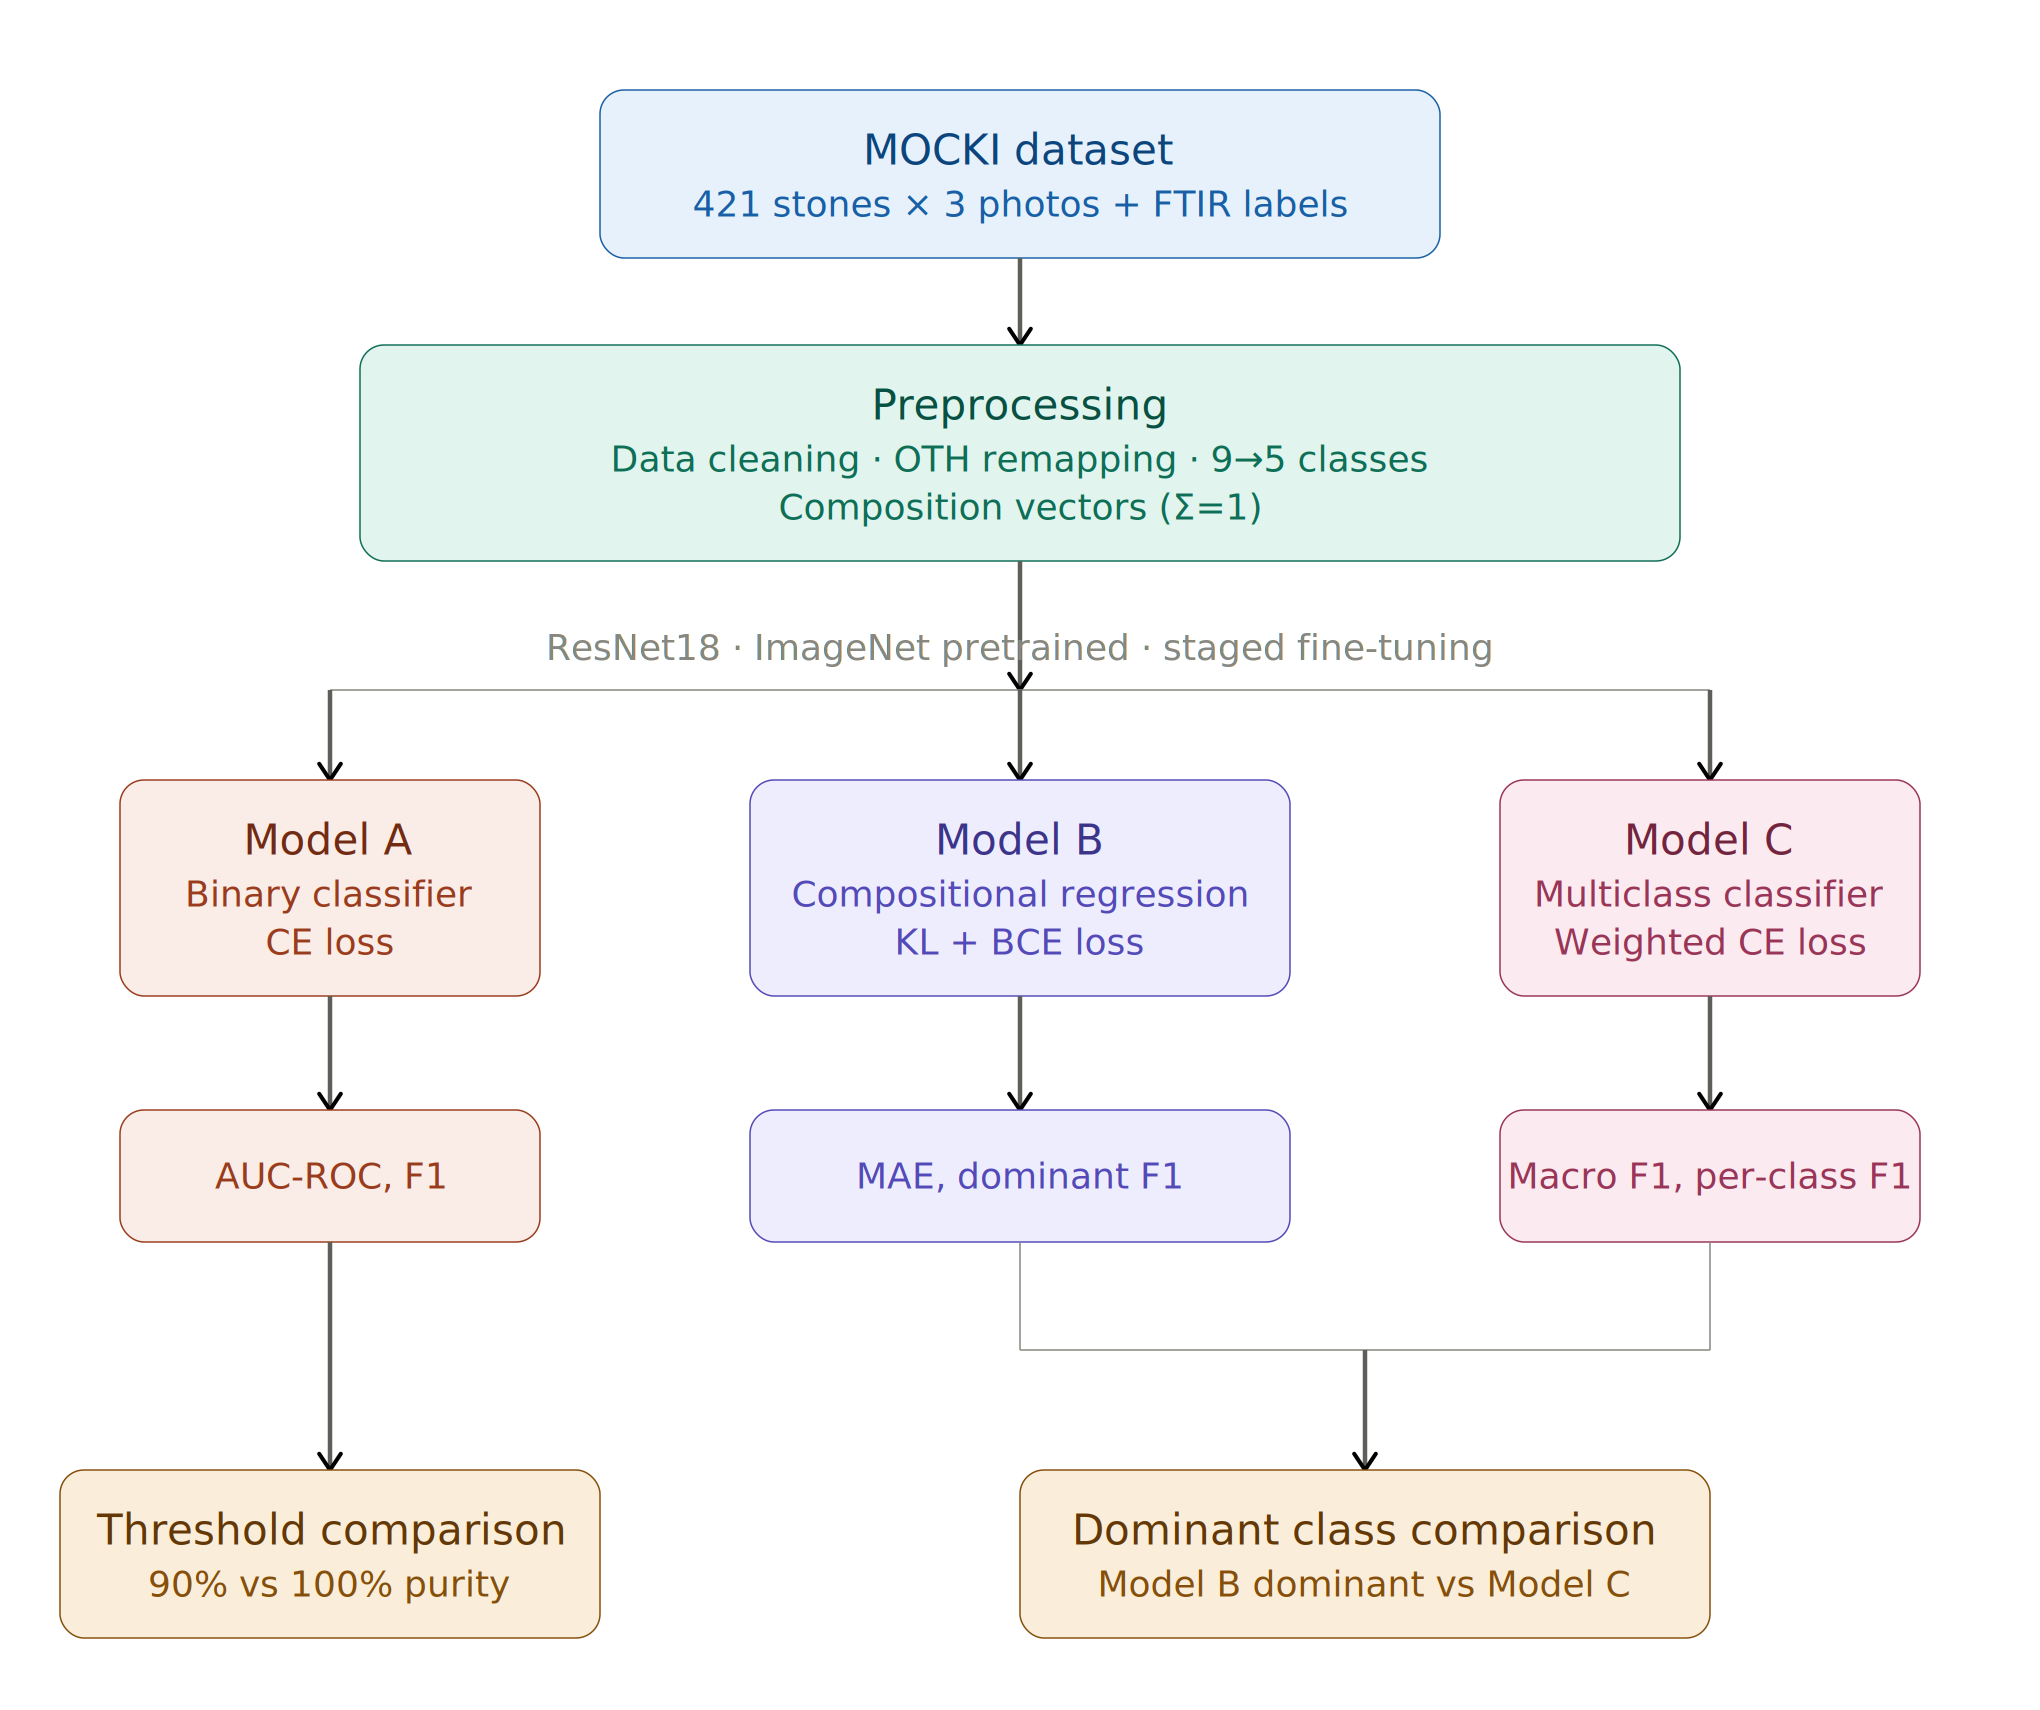
\includegraphics[width=0.8\textwidth]{figures/workflow_v3_3.png}
    \caption{\textbf{Overview of the study design.} ...}
    \label{fig:workflow}
\end{figure*}

\subsection*{Dataset}

\subsubsection*{Stone collection and imaging}

The dataset consists of 301 kidney stone fragments collected at Amsterdam UMC (VUmc) as part of the MOCKI study. Each fragment was photographed ex vivo immediately after retrieval using a standardised imaging protocol, yielding three photographs per stone (903 images in total). Stones were placed on a black background and photographed under controlled lighting conditions with a digital camera. Two stones (S168 and S301) were excluded due to missing FTIR labels, leaving 299 stones (897 images) for analysis.

\subsubsection*{FTIR composition labels}

Mineral composition was determined by FTIR spectroscopy following standard morpho-constitutional analysis \cite{Daudon2016}. The analysis produces continuous percentage values for each mineral component present in the stone. The raw FTIR output contains nine mineral classes.

\subsubsection*{Data preprocessing}

Raw data was extracted from the clinical Excel file via a reproducible preprocessing pipeline (\texttt{01\_data\_prep.py}). Several data quality issues were addressed. First, fragment identifiers were forward-filled across photo rows, as only the first photo of each stone carried the identifier in the original spreadsheet. Second, known data-entry errors in the percentage columns were corrected based on clinical verification (six stones: S14, S32, S44, S242--S244). Third, photo identifiers with formatting inconsistencies (missing prefixes, single-letter abbreviations) were standardised. Fourth, trailing whitespace in component labels was stripped to resolve parsing errors.

\subsubsection*{Class consolidation and OTH remapping}

The nine raw FTIR mineral classes were consolidated into six target classes through a two-stage remapping procedure. In the first stage, stones labelled as ``OTH'' (other) were examined using the FTIR sub-identification field recorded during analysis. Spelling variants were normalised, and chemically identifiable minerals were reassigned to the appropriate target class: sodium hydrogen urate hydrate (16 stones), monoammonium urate (7), and uric acid dihydrate (2) were assigned to UA; calcium-magnesium phosphate (3 stones) was assigned to CaP; and newberyite (1 stone) was assigned to MAP. The remaining OTH stones---calcite (9), protein/albumin (10), and xanthine (5)---were retained as OTH because they lack a clear chemical relationship to any of the major classes.

In the second stage, the standard component codes were merged into the final six classes:
\begin{itemize}
    \item \textbf{CaOx}: calcium oxalate monohydrate (COM) + calcium oxalate dihydrate (COD)
    \item \textbf{CaP}: carbonated hydroxyapatite (CHP) + dihydrate (CHPD) + magnesium-substituted (CMP)
    \item \textbf{UA}: uric acid (including remapped urate salts)
    \item \textbf{MAP}: struvite (magnesium ammonium phosphate, including remapped newberyite)
    \item \textbf{CYS}: cystine
    \item \textbf{OTH}: remaining minority minerals (calcite, protein, xanthine)
\end{itemize}

For Models B and C, the OTH class was excluded because it is chemically heterogeneous and too small (4 pure stones at the 90\% threshold) to train or evaluate reliably. After excluding stones whose dominant class was OTH, the remaining dataset for these models consisted of 5 target classes across 295 stones.

\subsubsection*{Composition vectors}

For each stone, a composition vector was constructed by summing the FTIR percentages across all positions (primary, secondary, tertiary) into the corresponding target class bucket. Any residual mass was redistributed proportionally so that each stone's composition vector sums to exactly 1.0. This normalised vector serves as the regression target for Model B and provides the dominant class label (via argmax) for Model C.

\subsubsection*{Purity labelling}

Stones with a single class comprising 100\% of the composition were designated \textit{pure}; all others were designated \textit{mixed}. This strict threshold was chosen in consultation with the urologists at Amsterdam UMC, who consider any detectable mixture clinically relevant. Prior literature has used a more lenient threshold of 90\% \cite{Kim2022}; to enable comparison, we evaluate Model A at both the 100\% and 90\% thresholds and report the effect on classification performance.

\subsubsection*{Data splitting}

All splits were performed at the stone level to prevent data leakage across the three photographs of the same stone. A held-out test set of 20\% of stones was reserved before cross-validation, using stratified sampling on the dominant mineral class. The remaining 80\% was split into five folds using stratified $k$-fold cross-validation. Model selection and hyperparameter tuning were performed exclusively on the cross-validation folds; the test set was used only for final evaluation.

\subsection*{Image preprocessing}

Input images were resized to $224 \times 224$ pixels. Before normalisation, a background masking step was applied: pixels whose mean RGB intensity fell below a threshold (20/255) were zeroed out. This prevents the model from learning features of the black imaging plate rather than the stone surface. After masking, pixel values were normalised using ImageNet channel statistics (mean = [0.485, 0.456, 0.406], std = [0.229, 0.224, 0.225]).

During training, data augmentation was applied to increase the effective dataset size and improve generalisation. Augmentations included random horizontal and vertical flips (each with probability 0.5), random rotation up to 45 degrees, and colour jitter (brightness $\pm$0.4, contrast $\pm$0.4, saturation $\pm$0.2). The choice of augmentations reflects the imaging setup: because stones are photographed ex vivo on a flat surface, orientation is arbitrary, justifying aggressive geometric augmentation. Colour jitter accounts for variation in lighting conditions across imaging sessions. No augmentation was applied during validation or testing.

\subsection*{Model architecture}

All three models use ResNet18 \cite{He2016} pretrained on ImageNet (IMAGENET1K\_V1 weights) as the backbone. ResNet18 is an 18-layer residual convolutional network with skip connections that enable stable gradient flow during training. We chose ResNet18 over ResNet50---used in most prior kidney stone classification studies \cite{LopezTiro2024, veltheer2025}---because the small dataset size ($\sim$300 stones) makes the larger model prone to overfitting despite regularisation.

The backbone's original classification head is replaced with an identity function, yielding a 512-dimensional feature vector from the global average pooling layer. A task-specific output head is attached to this vector for each model.

\subsubsection*{Model A: binary pure/mixed classifier}

Model A adds a dropout layer ($p = 0.5$) followed by a single linear layer mapping the 512-dimensional feature vector to two logits. The model is trained with cross-entropy loss:
\begin{equation}
    \mathcal{L}_{\text{CE}} = -\sum_{k=0}^{1} \mathbf{1}[y=k] \log \hat{p}_k
\end{equation}
where $y \in \{0, 1\}$ is the ground-truth label (0 = pure, 1 = mixed) and $\hat{p}_k$ is the softmax-normalised predicted probability for class $k$.

Stone-level predictions are obtained by averaging the predicted probability of the mixed class across the three images of the same stone, with a decision threshold of 0.5.

\subsubsection*{Model B: compositional regression}

Model B is the primary model of this study. It predicts a continuous five-dimensional composition vector $\hat{\mathbf{c}} \in \mathbb{R}^5$ representing the estimated fractional contribution of each mineral class (CaOx, CaP, UA, MAP, CYS). The architecture consists of a shared backbone feeding two output heads.

The \textit{composition head} is a single shared regression head: a linear layer mapping the 512-dimensional feature vector to 128 hidden units, followed by ReLU activation, dropout ($p = 0.5$), and a final linear layer producing 5 logits. These are passed through a softmax function to enforce the compositional simplex:
\begin{equation}
    \hat{c}_k = \frac{\exp(z_k)}{\sum_{j=1}^{5} \exp(z_j)}, \quad k = 1, \ldots, 5
\end{equation}
This ensures $\hat{\mathbf{c}} \geq 0$ and $\sum_k \hat{c}_k = 1$, making predictions directly comparable to FTIR-derived composition vectors. The softmax is used as a simplex constraint, not to produce class probabilities---this is a compositional regression problem, not a classification task.

The \textit{auxiliary presence head} independently predicts which mineral classes are present in a stone (fraction $> 0.05$). It shares the same backbone features and has an identical architecture (512 $\to$ 128 $\to$ ReLU $\to$ dropout $\to$ 5), but its outputs pass through independent sigmoids rather than a joint softmax. The presence head provides a secondary training signal that encourages the shared backbone to learn features sensitive to minority components.

The total loss is a weighted combination of two terms:
\begin{equation}
    \mathcal{L}_{\text{total}} = \mathcal{L}_{\text{comp}} + \lambda \cdot \mathcal{L}_{\text{pres}}
\end{equation}
where $\lambda = 0.3$. The composition loss is Kullback--Leibler divergence between the predicted and true composition distributions:
\begin{equation}
    \mathcal{L}_{\text{comp}} = \text{KL}(\mathbf{c} \| \hat{\mathbf{c}}) = \sum_{k=1}^{5} c_k \log \frac{c_k}{\hat{c}_k}
\end{equation}
KL divergence is a natural loss for distributions on the simplex: it penalises confidently wrong predictions more heavily than $L_1$ or MSE, which treat all errors equally regardless of how the remaining probability mass is distributed. The presence loss is binary cross-entropy applied independently to each class:
\begin{equation}
    \mathcal{L}_{\text{pres}} = -\frac{1}{5} \sum_{k=1}^{5} \left[ t_k \log \sigma(\hat{t}_k) + (1 - t_k) \log (1 - \sigma(\hat{t}_k)) \right]
\end{equation}
where $t_k = \mathbf{1}[c_k > 0.05]$ is the binary presence target and $\sigma(\hat{t}_k)$ is the sigmoid-activated output of the presence head.

Stone-level predictions are obtained by averaging the predicted composition vectors across the three images of the same stone, followed by re-normalisation to sum to 1.

\subsubsection*{Model C: multiclass classifier}

Model C uses the same backbone and head architecture as Model A (dropout + linear), but outputs five logits corresponding to the five mineral classes. The model is trained with class-weighted cross-entropy loss:
\begin{equation}
    \mathcal{L}_{\text{CE}} = -\sum_{k=1}^{5} w_k \cdot \mathbf{1}[y=k] \log \hat{p}_k
\end{equation}
where $y$ is the dominant class label (argmax of the FTIR composition vector) and $w_k = N / (K \cdot n_k)$ is the inverse-frequency weight for class $k$ ($N$ is the total training count, $K = 5$, and $n_k$ is the count of class $k$ in the training set). Class weighting was applied because the dataset is heavily imbalanced: CaOx accounts for roughly 43\% of stones while MAP and CYS together represent less than 14\%.

Model C serves as a direct baseline for Model B: both models can be evaluated on dominant class prediction accuracy, allowing a controlled comparison between predicting continuous compositions and directly classifying the dominant component.

Stone-level predictions are obtained by averaging the softmax class probability vectors across the three images and taking the argmax.

\subsection*{Training procedure}

All models were trained using a two-phase staged fine-tuning strategy.

In Phase 1 (frozen backbone), the ResNet18 backbone weights were frozen and only the output head was trained for 5 epochs using the Adam optimiser with a learning rate of $1 \times 10^{-3}$ and weight decay of $1 \times 10^{-3}$. This allows the head to learn a useful mapping from ImageNet features to the target output before the backbone weights are perturbed. Only the head receives gradient updates during this phase.

In Phase 2 (full fine-tuning), the entire network was unfrozen and trained end-to-end. Two parameter groups were defined with separate learning rates: the backbone at $1 \times 10^{-5}$ and the head at $1 \times 10^{-3}$. This differential learning rate prevents large gradient updates from destroying the pre-trained backbone representations during early fine-tuning. Phase 2 ran for up to 20 epochs (Model A, Model C) or 25 epochs (Model B), with early stopping based on validation loss (patience = 5 for Models A and C, patience = 7 for Model B). Upon entering Phase 2, the best validation loss tracker was reset, allowing the model to be evaluated against a fair Phase 2 baseline.

A batch size of 64 was used throughout. Training was performed on an NVIDIA A100 GPU (80 GB) on the Snellius HPC cluster (SURF). All random seeds were fixed (seed = 42) for reproducibility.

Five-fold cross-validation was used to estimate performance. The final reported metrics are the mean and standard deviation across folds.

\subsection*{Evaluation metrics}

\subsubsection*{Model A}

Binary classification performance was assessed using the area under the receiver operating characteristic curve (AUC-ROC), precision, recall, and F1 score. All metrics are reported at the stone level after mean-probability aggregation.

\subsubsection*{Model B}

Compositional regression performance was evaluated using mean absolute error (MAE) per mineral class and overall, computed at the stone level between predicted and FTIR-derived composition vectors. To allow direct comparison with Model C, Model B predictions were converted to dominant class predictions by taking $\arg\max_k \hat{c}_k$, and macro-F1 and per-class F1 were computed. Presence detection performance of the auxiliary head was evaluated separately using per-class precision, recall, and F1.

\subsubsection*{Model C}

Multiclass classification performance was assessed using macro-averaged F1 score and per-class F1 score, all at the stone level.

\subsection*{Code and data availability}

All pipeline scripts, configuration files, and training code are publicly available at \url{https://github.com/Dirkdeboer/umc_thesis}. Raw images and FTIR labels are held at Amsterdam UMC (VUmc) and are not publicly available but may be accessible on request for academic research purposes.

\bibliographystyle{plain}
\bibliography{references}

\end{document}